% !TEX root = ../../main.tex
\section{Sơ đồ ERD ở mức Logic (Logical ERD Diagram)}
\label{sec:2_4_so_do_erd_logic}

Sau khi hoàn tất quá trình chuyển đổi từ mô hình thực thể -- liên kết mở rộng (EERD) sang mô hình dữ liệu quan hệ (Mục~\ref{sec:2_1_quy_tac_chuyen_doi}), xây dựng cấu trúc 22 lược đồ quan hệ logic (Mục~\ref{sec:2_2_luoc_do_quan_he}) và chuẩn hóa dữ liệu triệt để đạt chuẩn BCNF/3NF (Mục~\ref{sec:2_3_chuan_hoa_du_lieu}), sơ đồ ERD ở mức Logic (Logical Entity-Relationship Diagram) được xây dựng nhằm cung cấp một bức tranh toàn cảnh trực quan, thể hiện đầy đủ các bảng dữ liệu, khóa chính (PK), khóa ngoại (FK) và mạng lưới liên kết quan hệ trong toàn bộ hệ thống \textbf{FamilyConnect}.

\subsection{Tổng quan Sơ đồ ERD mức Logic}

Khác với sơ đồ quan niệm ở Chương 1 (chủ yếu trừu tượng hóa các thực thể và loại mối kết hợp), sơ đồ ERD mức Logic phản ánh chính xác kiến trúc cơ sở dữ liệu sẵn sàng cho giai đoạn cài đặt vật lý:
\begin{itemize}
    \item \textbf{Cấu trúc bảng (Tables \& Columns):} Toàn bộ 22 bảng dữ liệu tương ứng với 22 thực thể và mối quan hệ được chuẩn hóa theo quy ước đặt tên \texttt{snake\_case}, liệt kê rõ danh sách các thuộc tính trường kèm kiểu dữ liệu logic.
    \item \textbf{Cơ chế định danh và liên kết (PK \& FK):} Xác định rõ Khóa chính (Primary Key -- PK) của từng bảng, các Khóa ngoại (Foreign Key -- FK) tham chiếu và các ràng buộc đơn nhất (\texttt{UNIQUE}) ép quan hệ $1:1$.
    \item \textbf{Giải quyết mối quan hệ nhiều--nhiều ($M:N$):} Toàn bộ các quan hệ $M:N$ quan niệm đã được chuyển đổi thành các bảng trung gian (Junction Tables) liên kết với hai bảng cha thông qua các cặp khóa ngoại tương ứng.
    \item \textbf{Biểu diễn quan hệ đệ quy và kế thừa:} Mô hình hóa quan hệ tự tham chiếu huyết thống phụ mẫu ($1:N$) và quan hệ hôn phối lịch sử ($M:N$) trên cùng một thực thể, cũng như phương pháp phân rã bảng con kế thừa cho thành viên nội tộc và dâu/rể.
\end{itemize}

\begin{figure}[htbp]
    \centering
    \makebox[\textwidth][c]{%
        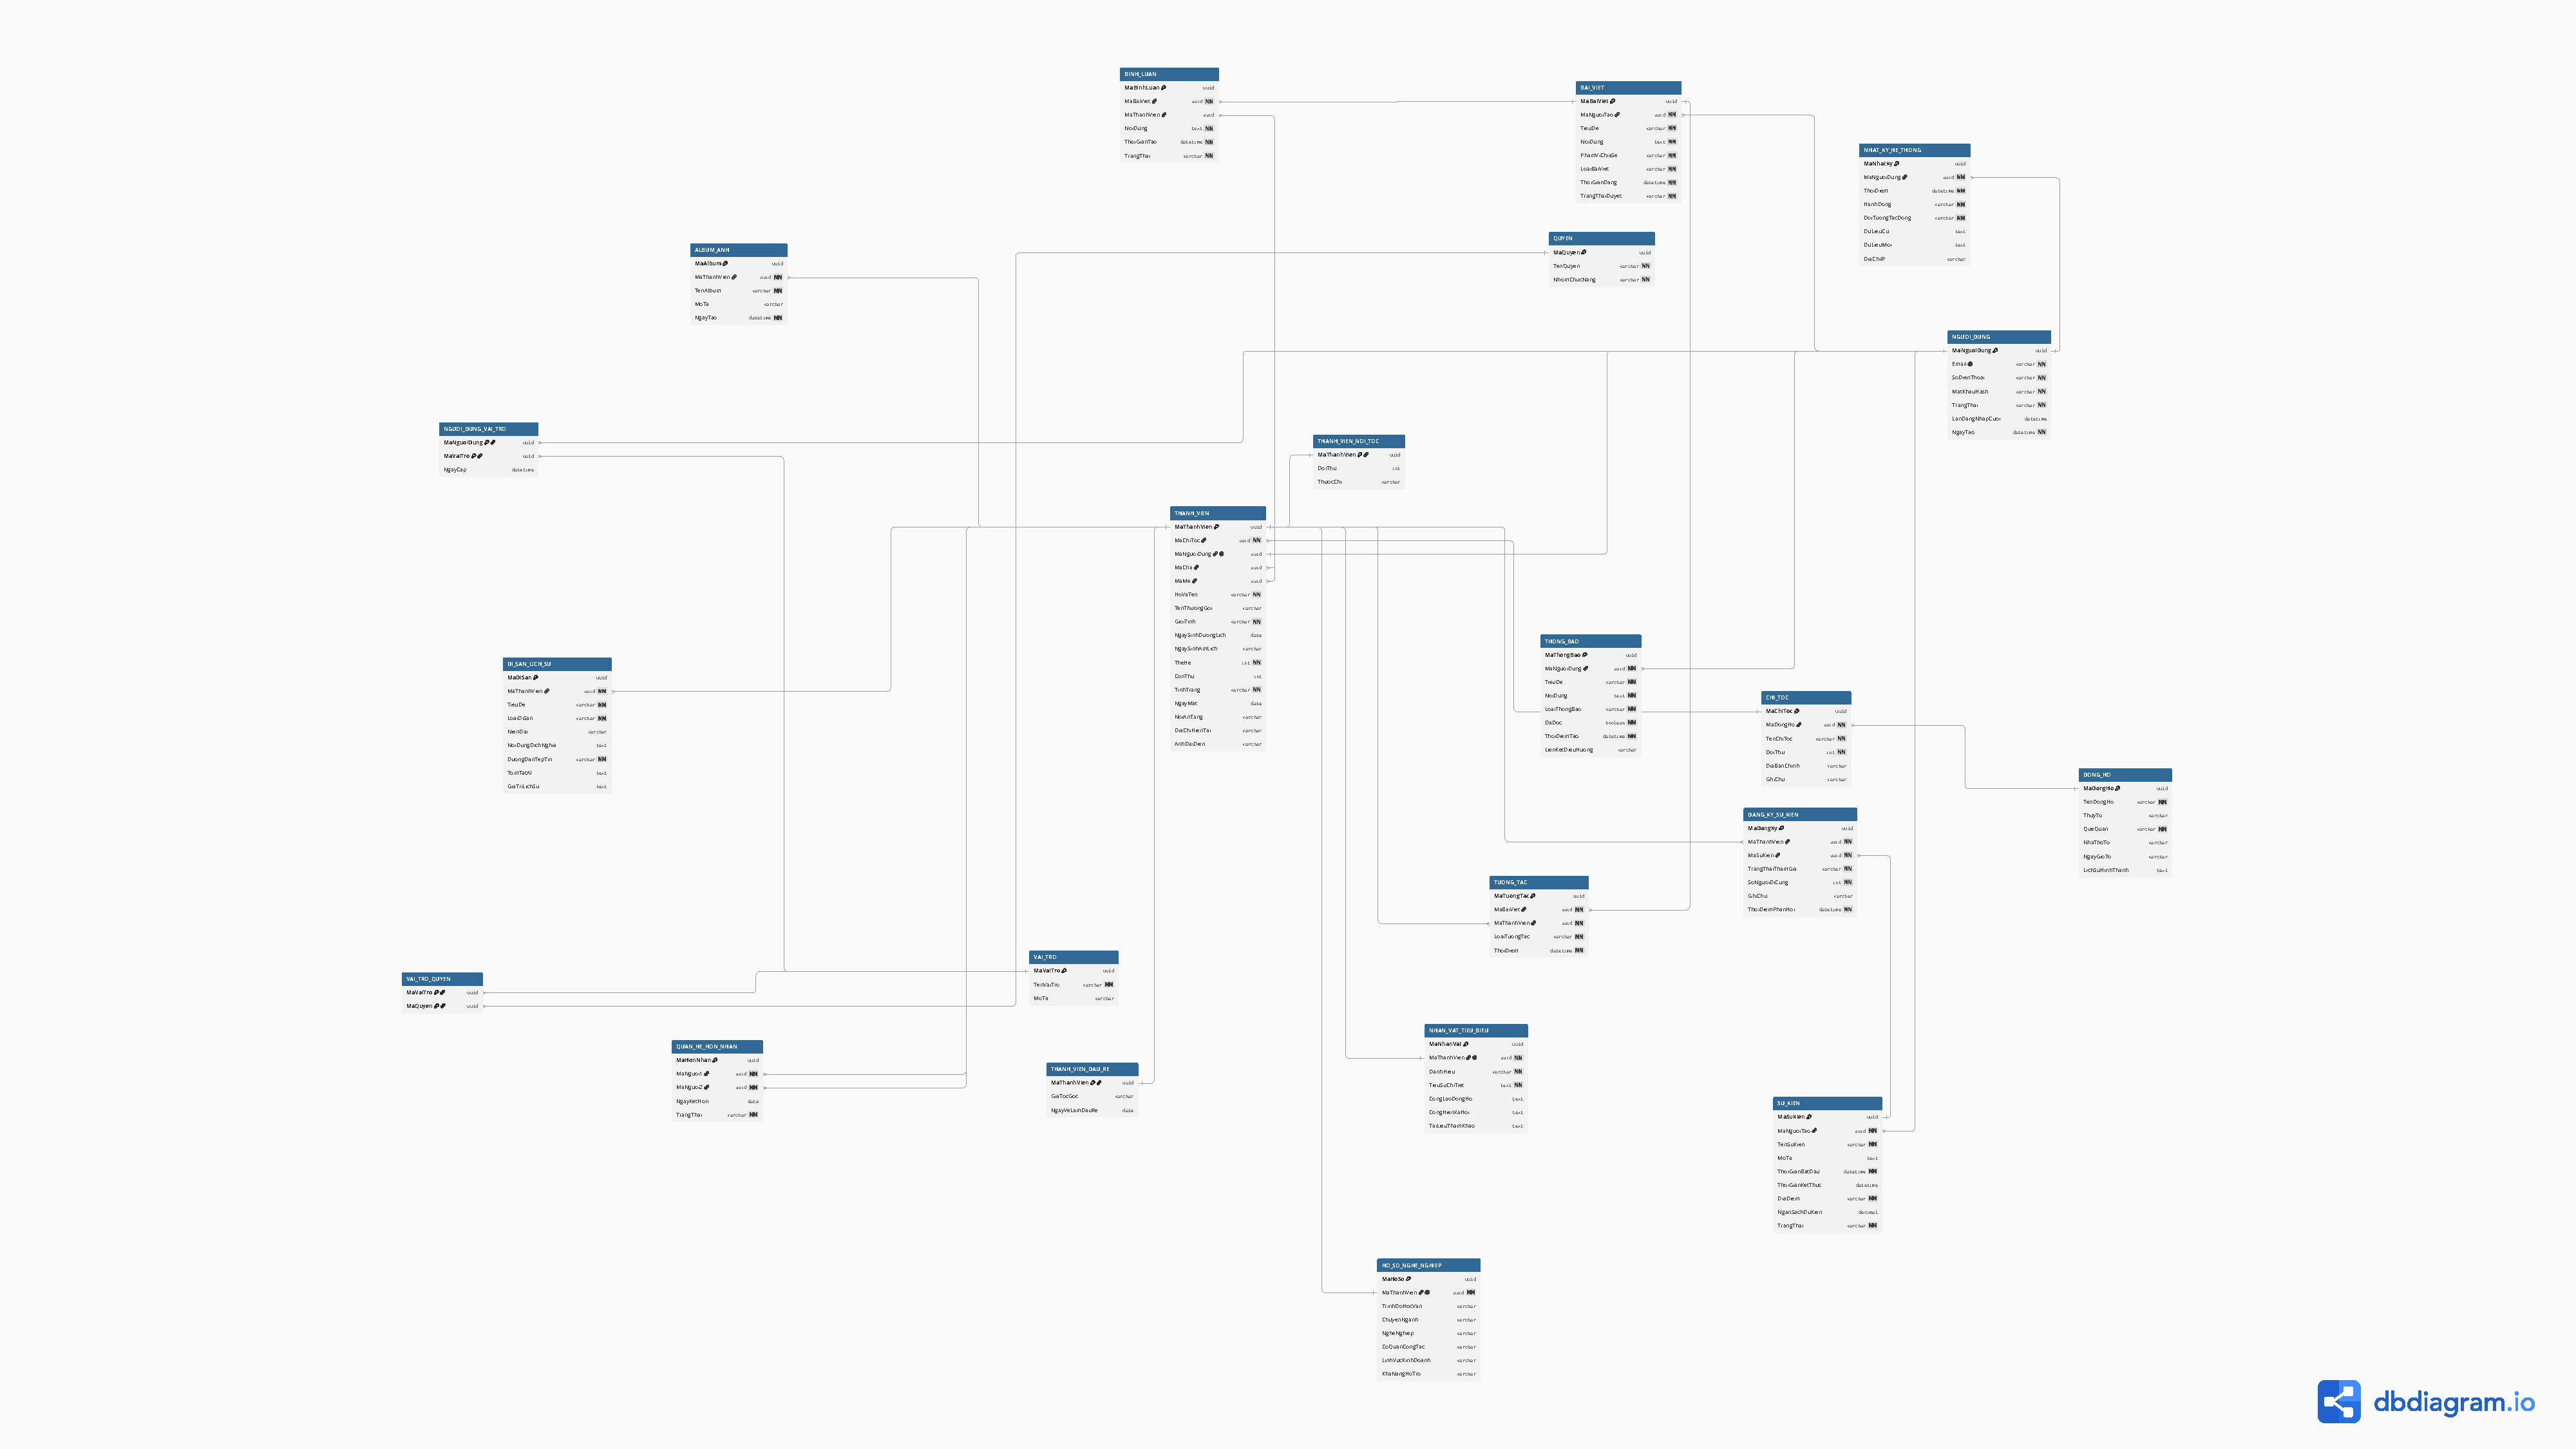
\includegraphics[page=1, trim={295pt 50pt 295pt 45pt}, clip, width=1.06\textwidth]{figures/erd_logic.pdf}%
    }
    \caption{Sơ đồ ERD ở mức Logic của hệ thống FamilyConnect (Toàn cảnh 22 bảng)}
    \label{fig:erd_logic_diagram}
\end{figure}

\noindent\textbf{Liên kết mô hình tương tác trực tuyến:} Nhằm hỗ trợ việc theo dõi chi tiết các trường, kiểu dữ liệu và mối liên kết trực quan giữa 22 bảng ở độ phân giải gốc cao nhất, sơ đồ được xuất bản trực tuyến tại: \url{https://dbdiagram.io/d/Test-6ab17faa9ba2420e18d44291}.

\subsection{Phân tích kiến trúc liên kết theo phân hệ nghiệp vụ}

Dựa trên sơ đồ ERD mức Logic (Hình~\ref{fig:erd_logic_diagram}), cấu trúc quan hệ giữa 22 bảng được tổ chức thành 4 phân hệ chức năng đồng bộ:

\subsubsection{1. Phân hệ Tài khoản, Xác thực \& Phân quyền RBAC}
\begin{itemize}
    \item \textbf{Bảng trung tâm:} \texttt{nguoi\_dung} (PK: \texttt{ma\_nguoi\_dung}) đóng vai trò quản lý tài khoản xác thực độc lập.
    \item \textbf{Phân quyền đa cấp ($M:N$):} Được tổ chức chặt chẽ thông qua hai bảng trung gian:
    \begin{itemize}
        \item Bảng \texttt{nguoi\_dung\_vai\_tro} lưu vết việc gán vai trò (\texttt{vai\_tro}) cho người dùng kèm mốc thời gian cấp (\texttt{ngay\_cap}).
        \item Bảng \texttt{vai\_tro\_quyen} phân rã các hành động nghiệp vụ chi tiết (\texttt{quyen}) cho từng vai trò cụ thể.
    \end{itemize}
    \item \textbf{Nhật ký kiểm toán:} Bảng \texttt{nhat\_ky\_he\_thong} liên kết trực tiếp với \texttt{nguoi\_dung} qua FK \texttt{ma\_nguoi\_dung} (\texttt{ON DELETE CASCADE}) để ghi vết mọi hoạt động truy cập và biến động dữ liệu.
\end{itemize}

\subsubsection{2. Phân hệ Cốt lõi: Gia tộc, Chi tộc \& Phả hệ Huyết thống}
\begin{itemize}
    \item \textbf{Cây tổ chức dòng họ:} Thiết lập phân cấp chặt chẽ $1:N$ từ \texttt{dong\_ho} $\to$ \texttt{chi\_toc} $\to$ \texttt{thanh\_vien}. Mọi thành viên bắt buộc phải thuộc về một chi tộc cụ thể.
    \item \textbf{Thực thể trung tâm \texttt{thanh\_vien}:} Là tâm điểm kết nối của toàn bộ cơ sở dữ liệu:
    \begin{itemize}
        \item Liên kết tùy chọn $1:1$ với tài khoản hệ thống: FK \texttt{ma\_nguoi\_dung} ($\to$ \texttt{nguoi\_dung}) phục vụ nghiệp vụ nhận hồ sơ gia phả cá nhân (\textit{Profile Claiming}).
        \item Quan hệ đệ quy huyết thống ($1:N$): Hai cột FK \texttt{ma\_cha} và \texttt{ma\_me} tự tham chiếu về chính \texttt{thanh\_vien.ma\_thanh\_vien} (\texttt{ON DELETE SET NULL}), hỗ trợ thuật toán duyệt cây gia phả nhiều thế hệ.
        \item Quan hệ hôn phối ($M:N$): Bảng trung gian \texttt{quan\_he\_hon\_nhan} chứa cặp FK (\texttt{ma\_nguoi1}, \texttt{ma\_nguoi2}) đều tham chiếu về \texttt{thanh\_vien}, lưu giữ trạng thái và mốc thời gian kết hôn lịch sử.
    \end{itemize}
    \item \textbf{Bảng kế thừa thực thể con ($1:1$):} Hai bảng \texttt{thanh\_vien\_}\allowbreak\texttt{noi\_toc} và \texttt{thanh\_vien\_}\allowbreak\texttt{dau\_re} dùng chung PK \texttt{ma\_thanh\_vien} đồng thời đóng vai trò là FK tham chiếu về bảng cha \texttt{thanh\_vien} (\texttt{CASCADE}), phân tách rành mạch thuộc tính riêng của người ruột thịt và dâu/rể.
    \item \textbf{Hồ sơ nghề nghiệp:} Bảng phụ \texttt{ho\_so\_nghe\_nghiep} gắn với \texttt{thanh\_vien} theo tỷ lệ $1:1$ bắt buộc thông qua ràng buộc \texttt{UNIQUE} trên FK \texttt{ma\_thanh\_vien}.
\end{itemize}

\subsubsection{3. Phân hệ Mạng xã hội Gia đình, Sự kiện \& Truyền thông}
\begin{itemize}
    \item \textbf{Bảng tin \& Tương tác:} Bảng \texttt{bai\_viet} nhận FK \texttt{ma\_nguoi\_tao} từ \texttt{nguoi\_dung}. Các phản hồi thảo luận được lưu ở bảng phụ \texttt{binh\_luan} (FK: \texttt{ma\_bai\_viet}). Tương tác cảm xúc được xử lý qua bảng trung gian \texttt{tuong\_tac} kết nối giữa \texttt{thanh\_vien} và \texttt{bai\_viet}.
    \item \textbf{Kho lưu trữ hình ảnh:} Bảng \texttt{album\_anh} trực thuộc quyền quản lý của thành viên gia đình thông qua FK \texttt{ma\_thanh\_vien}.
    \item \textbf{Tổ chức sự kiện \& Điểm danh RSVP:} Bảng \texttt{su\_kien} quản lý các buổi lễ giỗ, họp mặt gia tộc. Việc đăng ký tham dự được thực thể hóa qua bảng trung gian \texttt{dang\_ky\_su\_kien} chứa các cặp khóa ngoại (\texttt{ma\_thanh\_vien}, \texttt{ma\_su\_kien}) cùng số lượng người đi cùng và trạng thái điểm danh.
    \item \textbf{Thông báo đa kênh:} Bảng \texttt{thong\_bao} phụ thuộc tồn tại vào tài khoản người nhận (\texttt{nguoi\_dung}).
\end{itemize}

\subsubsection{4. Phân hệ Di sản số \& Vinh danh Tiền nhân}
\begin{itemize}
    \item \textbf{Di sản tư liệu lịch sử:} Bảng \texttt{di\_san\_lich\_su} lưu giữ các văn bản, gia phả cổ, sắc phong do thành viên tải lên (FK: \texttt{ma\_thanh\_vien}).
    \item \textbf{Vinh danh danh nhân gia tộc:} Bảng phụ \texttt{nhan\_vat\_tieu\_bieu} tôn vinh các tiền nhân có công trạng lớn, liên kết $1:1$ với \texttt{thanh\_vien} qua FK \texttt{ma\_thanh\_vien} mang ràng buộc \texttt{UNIQUE}.
\end{itemize}

\subsection{Đánh giá tính nhất quán và toàn vẹn của mô hình}

Sơ đồ ERD ở mức Logic thể hiện tính khoa học và chuẩn mực cao trong thiết kế CSDL quan hệ:
\begin{enumerate}
    \item \textbf{Bảo toàn phụ thuộc hàm và không mất mát thông tin:} Toàn bộ 17 thực thể nghiệp vụ ban đầu cùng các mối kết hợp được bảo toàn 100\% khi phân rã thành 22 quan hệ.
    \item \textbf{Triệt tiêu dư thừa dữ liệu:} Tất cả các bảng trung gian giải quyết dứt điểm các mối kết hợp nhiều--nhiều, không tồn tại thuộc tính lặp hay phụ thuộc bắc cầu, đảm bảo chuẩn hóa dữ liệu tối ưu.
    \item \textbf{Toàn vẹn tham chiếu chặt chẽ:} Thiết lập tường minh các chính sách hành vi ngoại vi (\texttt{CASCADE}, \texttt{SET NULL}, \texttt{RESTRICT}) giúp cơ sở dữ liệu duy trì tính ổn định, sẵn sàng chuyển giao sang giai đoạn Thiết kế Vật lý trên hệ quản trị CSDL (Chương~\ref{chap:chuong3_vat_ly}).
\end{enumerate}
